\section*{Software-Design}
Die Software wurde mit UML modelliert. Zuerst wurden aus den Anforderungsdiagrammen Komponenten abgeleitet (siehe Abbildung \ref{fig:UMLKomponentendiagramm}).\\[1ex]

\begin{figure}[H]
\centering
	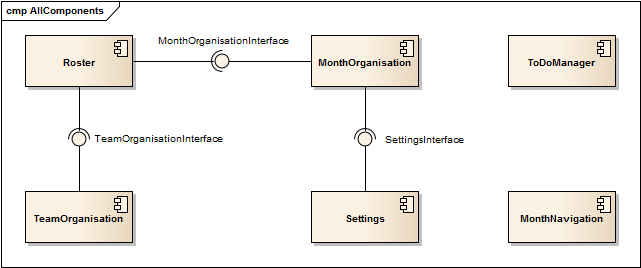
\includegraphics[width=1.0\textwidth]{../Images/Modell/UMLAllComponents.png}
	\caption[UML Komponentendiagramm]{UML Komponentendiagramm}
	\label{fig:UMLKomponentendiagramm}
\end{figure}

Daraufhin wurden Klassendiagramme entworfen. Als Beispiel ist das Klassendiagramm der Komponente \texttt{MonthOrganisation} in Abbildung \ref{fig:UMLComponentMonthOrganisation} gezeigt.\\[1ex]

\begin{figure}[H]
	\centering
	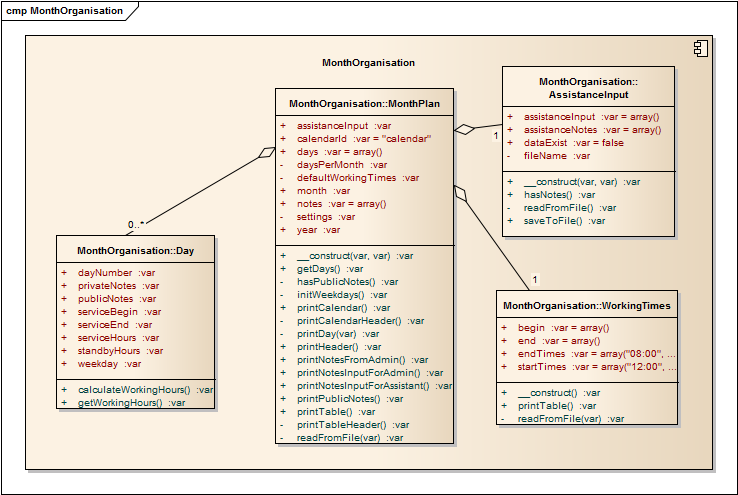
\includegraphics[width=1.0\textwidth]{../Images/Modell/UMLComponentMonthOrganisation.png}
	\caption{Klassendiagramm der Komponente \texttt{MonthOrganisation}}
	\label{fig:UMLComponentMonthOrganisation}
\end{figure}

\section*{Implementierung}
Der Assistenzplaner wurde mit PHP, HTML, CSS und JavaScript implementiert.